%
% green-beweis.tex
%
% (c) 2024 Prof Dr Andreas Müller
%
\begin{figure}
\centering
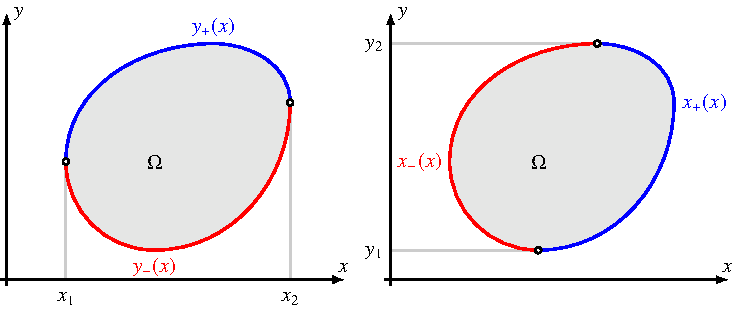
\includegraphics{chapters/040-felder/images/greenbeweis.pdf}
\caption{Beweis des Satzes von Green für ein Gebiet, welches durch
die Graphen zweier Funktionen $y_(x)$ und $y_+(x)$ 
berandet ist.
Alternativ kann das gleiche Gebiet auch durch die Graphen der Funktionen
$x_-(y)$ und $x_+(y)$ berandet werden.
Die Verwendung der beiden Berandungsarten für verschiedene Komponenten
in der Formel von Green ermöglicht den Beweis.
\label{buch:felder:fundamentallemma:fig:greenbeweis}}
\end{figure}
